In  this section, we report our experimental evaluation of our language. 
We focus on three benchmarks: the dice program that we compare with the  
test cases reported in the PRISM repository\footnote{\url{https://www.prismmodelchecker.org/casestudies/}}; 
the Bitcoin Proof of Work protocol and the Hybrid Casper protocol, 
presented in \cite{DBLP:journals/concurrency/BistarelliNGLMV23,DBLP:journals/distribledger/GallettaLMV23}.
For lack of space, we do not report the generated PRISM files, they can be found in the online repository \cite{repository}.
\subsection{The Dice Program}
 The first test case we focus on the Dice Program \cite{KY76}.
 The following program simulates a die using only unbiased coins. Starting from the initial vertex (state $s_0$), the process involves the iterative flipping of a coin. Upon obtaining heads, the upper branch is chosen, and in the case of tails, the lower branch is taken. This sequential process persists until the final determination of the die's value.
 In particular, the PRISM model uses two variables: 
 \begin{itemize}
	\item \codeprism{d}: This variable represents the value of the dice, ranging from 0 to 6. Initially, it is set to 0.
	\item \codeprism{STATE}: This variable is the state variable, ranging from 0 to 7. Initially, it is set to 0.
 \end{itemize}
 
 \vspace{-0.25cm}
 \begin{lstlisting}[style=chor-color,caption={Choreographic language for the Dice Program},captionpos=b,label={ex1-code}]
	$\ldots$
	{
	DiceProtocol0 $\coloneqq$  Dice $\rightarrow$ Dice : (+["0.5*1"] ; DiceProtocol1
						 +["0.5*1"] ;  DiceProtocol2)
	
	DiceProtocol1 $\coloneqq$ Dice $\rightarrow$ Dice : (+["0.5*1"] ; Dice $\rightarrow$ Dice : 
							(+["0.5*1"]  ; DiceProtocol1
							 +["0.5*1"]  "(d'=1)" ; DiceProtocol7)
					     +["0.5*1"] ;  Dice $\rightarrow$ Dice : 
							(+["0.5*1"]  "(d'=2)" ; DiceProtocol7
							 +["0.5*1"]  "(d'=3)" ; DiceProtocol7))
	$\ldots$
	DiceProtocol7 $\coloneqq$ Dice $\rightarrow$ Dice : (["1*1"] ; END)
	}
		
	\end{lstlisting}

The PRISM model produced by our method closely aligns with the original model with only minimal details that differ between the two.
Additionally, to ensure the generated program's accuracy, 
we evaluated whether the probability of reaching a state where the dice displays \texttt{d=k} for every possible \texttt{k} from 1 to 6 equals 1/6. Our simulations shown that the probabilities calculated by our generated model fully matched those from the original PRISM model. 

\begin{comment}
\subsection{Simple Peer-To-Peer Protocol}
This case study describes a simple peer-to-peer protocol based on BitTorrent\footnote{\url{https://www.prismmodelchecker.org/casestudies/peer2peer.php}}. The model comprises a set of clients trying to download a file that has been partitioned into $K$ blocks. Initially, there is one client that has already obtained all of the blocks and $N$ additional clients with no blocks. Each client can download a block from any of the others but they can only attempt four concurrent downloads for each block.\\
The code we analyze with $k=5$ and $N=4$ is reported in Listing \ref{ex2-code}.
\begin{lstlisting}[style=chor-color,caption={Choreographic language for the Peer-To-Peer Protocol.},captionpos=b,label={ex2-code}]
preamble
"ctmc"
"const double mu=2;"
"formula rate1=mu*(1+min(3,b11+b21+b31+b41));"
"formula rate2=mu*(1+min(3,b12+b22+b32+b42));"
"formula rate3=mu*(1+min(3,b13+b23+b33+b43));"
"formula rate4=mu*(1+min(3,b14+b24+b34+b44));"
"formula rate5=mu*(1+min(3,b15+b25+b35+b45));"
endpreamble

n = 4;
n = 4;

Client[i] $\rightarrow$ i in [1...n]
Client[i] : "b[i]1 : [0..1];", "b[i]2 : [0..1];", "b[i]3 : [0..1];", "b[i]4 : [0..1];", "b[i]5 : [0..1];" ;

{
PeerToPeer := Client[i] $\rightarrow$ Client[i]: 
			(+["rate1*1"]  "(b[i]1'=1)"$\&\&$" " . PeerToPeer
			 +["rate2*1"]  "(b[i]2'=1)"$\&\&$" " . PeerToPeer
			 +["rate3*1"]  "(b[i]3'=1)"$\&\&$" " . PeerToPeer
			 +["rate4*1"]  "(b[i]4'=1)"$\&\&$" " . PeerToPeer
			 +["rate5*1"]  "(b[i]5'=1)"$\&\&$" " . PeerToPeer)
}
	
\end{lstlisting}

Part of the generated PRISM code is shown in Listing \ref{ex2-gen} and it is faithful with what reported in the PRISM documentation. 
\begin{lstlisting}[style=prism-color,caption={Generated PRISM program for the Peer-To-Peer Protocol.},captionpos=b,label={ex2-gen}]
ctmc
const double mu=2;
formula rate1=mu*(1+min(3,b11+b21+b31+b41));
formula rate2=mu*(1+min(3,b12+b22+b32+b42));
formula rate3=mu*(1+min(3,b13+b23+b33+b43));
formula rate4=mu*(1+min(3,b14+b24+b34+b44));
formula rate5=mu*(1+min(3,b15+b25+b35+b45));

module Client1
	Client1 : [0..1] init 0;
	b11 : [0..1]; 
	b12 : [0..1]; 
	b13 : [0..1]; 
	b14 : [0..1]; 
	b15 : [0..1]; 

	[] (Client1=0)  $\rightarrow$ rate1 : (b11'=1)$\&$(Client1'=0); 
	[] (Client1=0)  $\rightarrow$ rate2 : (b12'=1)$\&$(Client1'=0); 
	[] (Client1=0)  $\rightarrow$ rate3 : (b13'=1)$\&$(Client1'=0); 
	[] (Client1=0)  $\rightarrow$ rate4 : (b14'=1)$\&$(Client1'=0); 
	[] (Client1=0)  $\rightarrow$ rate5 : (b15'=1)$\&$(Client1'=0); 
	
endmodule
	
\end{lstlisting}


In Figure \ref{ex2-res}, we compare the values obtained for the probability that all clients have received all blocks by time $0\leq T\leq 1.5$ both for our generated model and the model reported in the documentation.
\begin{figure}[h]
\centering
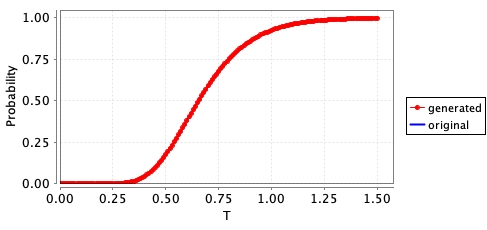
\includegraphics[scale=0.6]{example3-results.jpeg}	
\caption{Probability that clients received all the block before $T$, with $0\leq T \leq 1.5$.}
\label{ex2-res}
\end{figure}
\subsection{Random Graphs Protocol}
\begin{wrapfigure}[8]{l}{4cm}
	
\includegraphics[scale=0.7]{network.pdf}	
\end{wrapfigure} 
The second case study we report is the random graphs protocol presented in the PRISM documentation\footnote{\url{https://www.prismmodelchecker.org/casestudies/graph_connected.php}}.
It investigates the likelihood that a pair of nodes are connected in a
 random graph. More precisely, we take into account the the set of random graphs $G(n,p)$,
  i.e. the set of random graphs with $n$ nodes where the probability of there being an edge 
  between any two nodes equals $p$. 

  The model is divided in two parts: at the beginning the random graph is built.
Then the algorithm finds nodes that have a path to node 2 by searching for nodes for which one can reach (in one step) a node for which the existence of a path to node 2 has already been found.

The choreographic model is shown in Listing \ref{ex4-code}, while
in Listing \ref{ex4-gen}, we report only part of the generated PRISM module (the modules $M_2$, $M_3$ and $P_2$, $P_3$ are equivalent to, respectively, $M_1$ and $P_2$ and can be found in the repository\footnote{\url{https://github.com/adeleveschetti/choreography-to-PRISM}}).

\begin{lstlisting}[style=chor-color,breaklines=true, postbreak=\mbox{\textcolor{red}{$\hookrightarrow$}\space},caption={Choreographic language for the Random Graphs
	Protocol.},captionpos=b,label={ex4-code}]
preamble
"mdp"
"const double p;"
endpreamble

n = 3;

PC -> PC : " ";
M[i] -> i in [1...n]  M[i] : "varM[i] : bool;";
P[i] -> i in [1...n] P[i] : "varP[i] : bool;";

{
GraphConnected0 := 
	PC -> M[i] : (+["1*p"] " " "(varM[i]'=true)". END
		        +["1*(1-p)"] " " "(varM[i]'=false)". END)
	PC -> P[i] : (+["1*p"] " " "(varP[i]'=true)" . END
		        +["1*(1-p)"] " " "(varP[i]'=false)".
			if "(PC=6)&!varP[i]&((varP[i] & varM[i]) | (varM[i+1] & varP[i+2])) "@P[i] then {
				["1"]"(varP[i]'=true)"@P[i] . GraphConnected0
			}) 								  
}
\end{lstlisting}
\begin{lstlisting}[style=prism-color,caption={Generated PRISM program for the Random Graphs
	Protocol.},captionpos=b,label={ex4-gen}]
mdp
const double p;
	
module PC
   PC : [0..7] init 0;
	
   [DPPGR] (PC=0)  $\rightarrow$ 1 :  (PC'=1); 
   [YCJJG] (PC=1)  $\rightarrow$ 1 :  (PC'=2); 
   [TWGVA] (PC=2)  $\rightarrow$ 1 :  (PC'=3); 
   [NODPZ] (PC=3)  $\rightarrow$ 1 :  (PC'=4); 
   [FDALJ] (PC=4)  $\rightarrow$ 1 :  (PC'=5); 
   [DCKXC] (PC=5)  $\rightarrow$ 1 :  (PC'=6); 
endmodule

module M1
   M1 : [0..1] init 0;
   varM1 : bool; 

   [DPPGR] (M1=0)  $\rightarrow$ p :(varM1'=true)$\&$(M1'=0) + (1-p) :(varM1'=false)$\&$(M1'=0); 
endmodule	

$\ldots$

module P1
   P1 : [0..3] init 0;
   varP1 : bool; 

   [NODPZ] (P1=0)  $\rightarrow$ p:(varP1'=true)$\&$(P1'=0) + (1-p):(varP1'=false)$\&$(P1'=0); 
   [] (P1=0)$\&$(PC=6)$\&$!varP1&((varP1 $\&$ varM1) | (varM2$\&$ varP3))  
   				$\rightarrow$ 1 : (varP1'=true)$\&$(P1'=0); 
endmodule
$\ldots$
\end{lstlisting}

The model is very similar to the one presented in the PRISM repository, the main difference is that we use state variables also for the modules \texttt{P$_i$} and \texttt{M$_i$}, 
where in the original model they were not requires.
However, this does not affect the behaviour of the model, as the reader can notice from the results of the probability that nodes 1 and 2 are connected showed in Figure \ref{ex4-res}.
\begin{figure}[h]
\centering
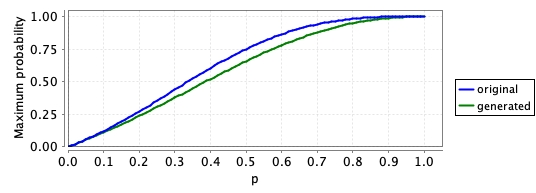
\includegraphics[scale=0.6]{example5-results.jpeg}	
\caption{Probability that the nodes 1 and 2 are connected.}
\label{ex4-res}
\end{figure}
\end{comment}
\subsection{Proof of Work Bitcoin Protocol}
\begin{comment}
\begin{wrapfigure}[11]{r}{4cm}
	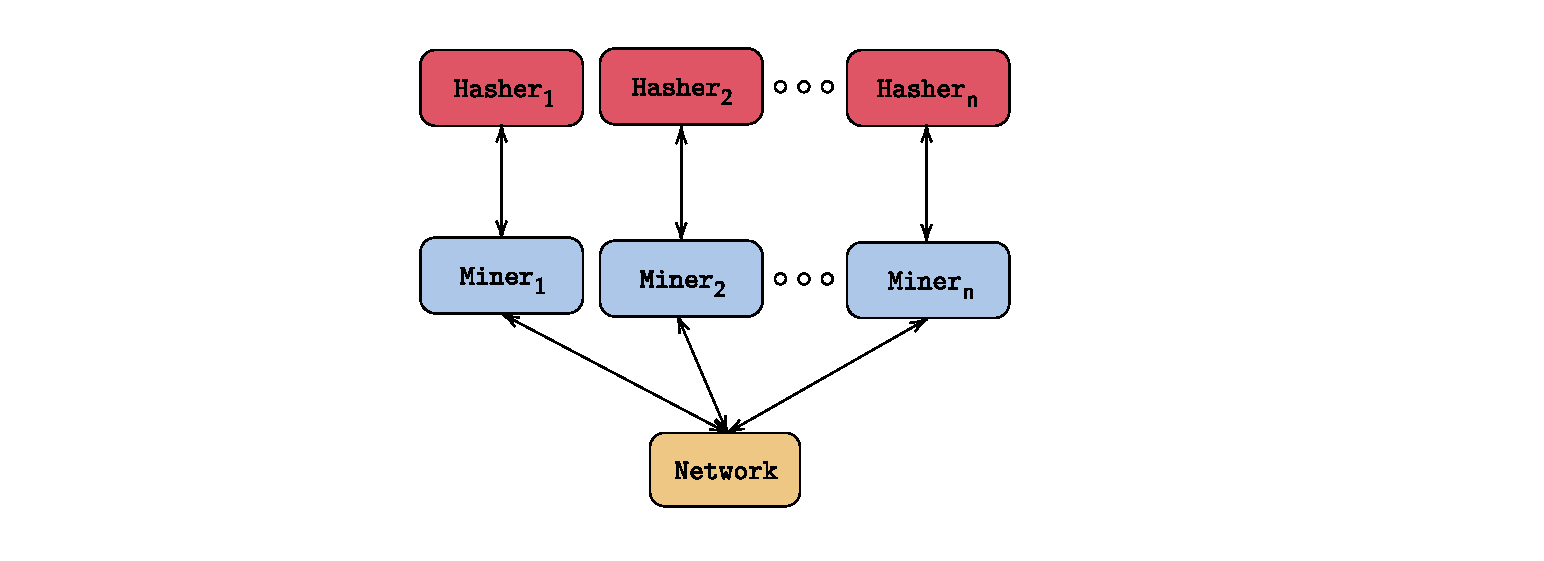
\includegraphics[scale=0.45]{bitcoin.pdf}	
\end{wrapfigure} 
\end{comment}
In \cite{DBLP:journals/concurrency/BistarelliNGLMV23}, the authors extended the PRISM model checker syntax to incorporate dynamic data types, enhancing its capabilities to model the Proof of Work protocol used in the Bitcoin blockchain \cite{bitcoin}. 

The Bitcoin system is modeled as a parallel composition of $n$ \emph{Miner} processes, $n$ \emph{Hasher} processes, and a process denoted as \emph{Network}. Specifically:
\begin{itemize}
\item \emph{Miner} processes replicate blockchain miners responsible for generating new blocks and appending them to their local ledger.
\item \emph{Hasher} processes simulate the process of solving the cryptographic puzzle.
\item \emph{Network} process models the broadcast communication among miners.
\end{itemize}
The choreographic model of the Proof of Work protocol is in Listing \ref{ex3-code}.
\begin{lstlisting}[style=chor-color,breaklines=true, postbreak=\mbox{\textcolor{red}{$\hookrightarrow$}\space},caption={Choreographic language for the Proof of Work Bitcoin Protocol},captionpos=b,label={ex3-code}]
$\ldots$
{PoW $\coloneqq$ Hasher[i] $\rightarrow$ Miner[i] :
(+["mR*hR[i]"]  " " "(b[i]'=createB(b[i],B[i],c[i]))&(c[i]'=c[i]+1)" ; 
	Miner[i] $\rightarrow$ Network : (["rB*1"] "(B[i]'=addBlock(B[i],b[i]))"   
		foreach(k!=i) "(set[k]'=addBlockSet(set[k],b[i]))"@Network;PoW)
 +["lR*hR[i]"] ; if "!isEmpty(set[i])"@Miner[i] then { 
  	   		["r"] "(b[i]'=extractBlock(set[i]))"@Miner[i] ;  
				Miner[i] $\rightarrow$ Network : 
					(["1*1"] "(setMiner[i]'=addBlockSet(setMiner[i],b[i]))"
		 			"(set[i]' = removeBlock(set[i],b[i]))";PoW) 
 		   }
 		   else{
 	   		if "canBeInserted(B[i],b[i])"@Miner[i] then { 
 	      			["1"] "(B[i]'=addBlock(B[i],b[i]))
				&(setMiner[i]'=removeBlock(setMiner[i],b[i]))"@Miner[i];PoW 
 	   		}
	   		else{PoW}
		   })} 
\end{lstlisting}
\begin{comment}
\begin{lstlisting}[style=prism-color,caption={Generated PRISM program for the Peer-To-Peer Protocol.},captionpos=b,label={ex3-gen}]
$\ldots$

module Miner1
   Miner1 : [0..7] init 0;
   b1 : block {m1,0;genesis,0} ; 
   B1 : blockchain [{genesis,0;genesis,0}]; 
   c1 : [0..N] init 0; 
   setMiner1 : list []; 

   [PZKYT] (Miner1=0)   $\rightarrow$  hR1 : (b1'=createB(b1,B1,c1))$\&$(c1'=c1+1)$\&$(Miner1'=1); 
   [EUBVP] (Miner1=0)   $\rightarrow$  hR1 :  (Miner1'=2); 
   [HXYKO] (Miner1=1)   $\rightarrow$  1 : (B1'=addBlock(B1,b1))$\&$(Miner1'=0); 
   [] (Miner1=2)$\&$!isEmpty(set1)  $\rightarrow$  r : (b1'=extractBlock(set1))$\&$(Miner1'=4); 
   [SRKSV] (Miner1=4)   $\rightarrow$  1 : (setMiner1' = addBlockSet(setMiner1 , b1))$\&$(Miner1'=0); 
   [] (Miner1=2)$\&$!(!isEmpty(set1))  $\rightarrow$  1 : (Miner1'=5); 
   [] (Miner1=5)$\&$canBeInserted(B1,b1)  $\rightarrow$  1 : (B1'=addBlock(B1,b1))$\&$(setMiner1'=removeBlock(setMiner1,b1))$\&$(Miner1'=0); 
   [] (Miner1=5)$\&$!(canBeInserted(B1,b1))  $\rightarrow$  1 : (Miner1'=0);

endmodule
$\ldots$
module Network
Network : [0..1] init 0;
   set1 : list []; 
   $\ldots$

   [HXYKO] (Network=0)  $\rightarrow$  1 : (set2'=addBlockSet(set2,b2))$\&$(set3'=addBlockSet(set3,b3))$\&$(set4'=addBlockSet(set4,b4))$\&$(Network'=0); 
   [SRKSV] (Network=0)  $\rightarrow$  1 : (set1' = removeBlock(set1,b1))$\&$(Network'=0); 
   $\ldots$

endmodule

module Hasher1
Hasher1 : [0..1] init 0;

[PZKYT] (Hasher1=0)  $\rightarrow$  mR :  (Hasher1'=0); 
[EUBVP] (Hasher1=0)  $\rightarrow$  lR :  (Hasher1'=0); 

endmodule
\end{lstlisting}

\end{comment}

\begin{wrapfigure}{r}{0.41\textwidth}
	\vspace{-0.75cm}
	\centering
	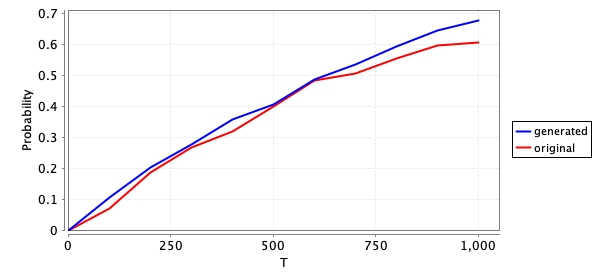
\includegraphics[scale=0.22]{example4-results.jpeg}	
	\vspace{-0.25cm}
	\caption{}
	\label{ex3-res}
	\vspace{-0.25cm}
	\end{wrapfigure}

The PRISM model we generated exhibits greater verbosity compared to the one presented in \cite{DBLP:journals/concurrency/BistarelliNGLMV23}. This difference arises from our approach of consistently generating the \texttt{else} branch for the \texttt{if-then-else} expression, resulting in an increased number of instructions.
Nevertheless, in the case of this specific test scenario, we proved that the experimental results remain unaffected, as reported in Figure \ref{ex3-res}.




\subsection{Hybrid Casper Protocol}
\begin{comment}
\begin{wrapfigure}[12]{l}{4.5cm}
	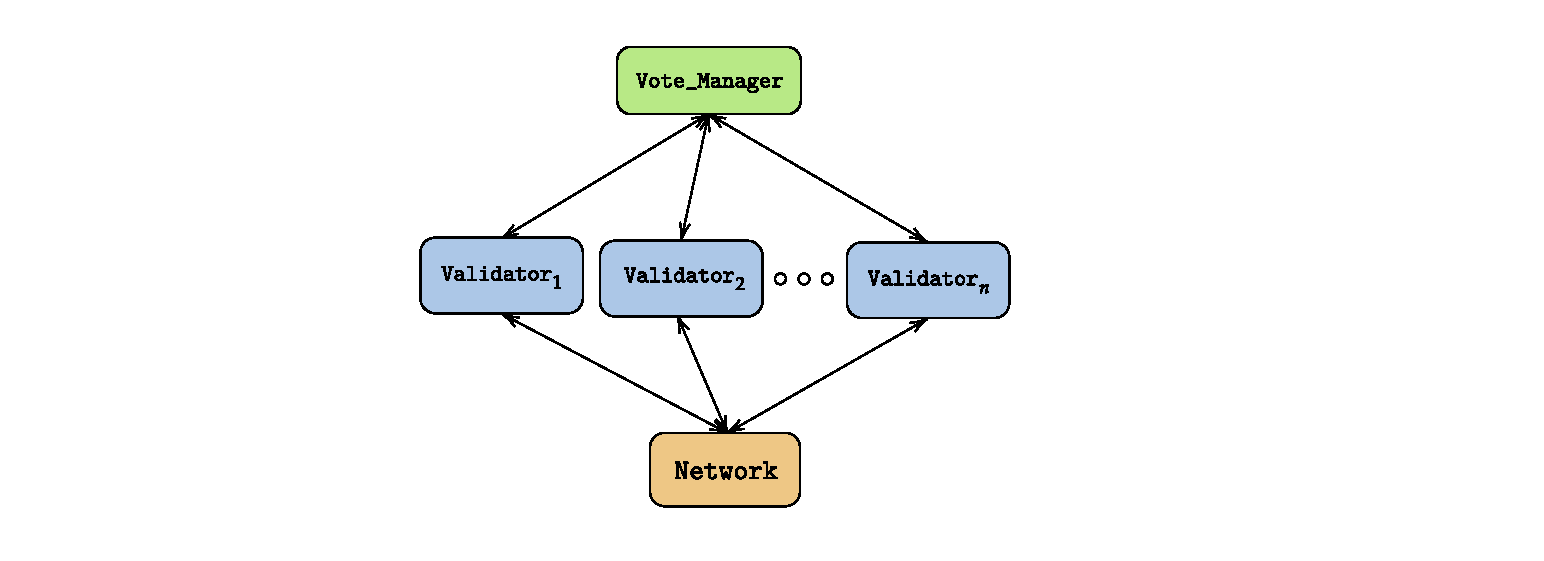
\includegraphics[scale=0.45]{ethereum.pdf}	
\end{wrapfigure} 
\end{comment}
We now present the Hybrid Casper Protocol \cite{DBLP:journals/distribledger/GallettaLMV23}. The Hybrid Casper protocol represents a hybrid consensus protocol for blockchains, merging features from both Proof of Work and Proof of Stake protocols. 

The modeling approach is very similar to the one used for the Proof of Work Bitcoin protocol. Specifically, the Hybrid Casper protocol is represented in PRISM as the parallel composition of $n$ \emph{Validator} modules, along with the modules \emph{Vote\_Manager} and \emph{Network}. Each \emph{Validator} module closely resembles the \emph{Miner} module from the previous protocol. The module \emph{Vote\_Manager} is responsible for storing maps containing votes for each block and computing associated rewards/penalties.
Part of the choreographic modelization is reported in Listing \ref{ex5-code}, the complete model can be found in \cite{repository}. 
\begin{lstlisting}[style=chor-color,tabsize=2,breaklines=true, postbreak=\mbox{\textcolor{red}{$\hookrightarrow$}\space},	caption={Choreographic language for the Hybrid Casper Protocol},captionpos=b,label={ex5-code}]
$\ldots$
{PoS := Validator[i] -> Validator[i] :
(+["mR*1"]  "(b[i]'=createB(b[i],L[i],c[i]))&(c[i]'=c[i]+1)"; 
	if "!(mod(getHeight(b[i]),EpochSize)=0)"@Validator[i] then{$\ldots$}
	else{
		Validator[i] -> Vote_Manager :(["1*1"]  "(Votes'=addVote(Votes,b[i],stake[i]))"; PoS)
	}
 +["hR*1"]  ; if "!isEmpty(set[i])"@Validator[i] then { $\dots$ }
 							else{ PoS }
 +["rC*1"] $\ldots$}

\end{lstlisting}
\begin{comment}
\begin{lstlisting}[style=prism-color,caption={Generated PRISM program for the Hybrid Casper	Protocol.},captionpos=b,label={ex5-gen}]
module Validator1
   $\ldots$
	
   [] (Validator1=0)  $\rightarrow$  mR : (b1'=createB(b1,L1,c1))$\&$(c1'=c1+1)&(Validator1'=1); 
   [] (Validator1=0)  $\rightarrow$  lR :  (Validator1'=2); 
   [] (Validator1=0)$\&$(!isEmpty(listCheckpoints1))  $\rightarrow$  
   	rC : (lastCheck1'=extractCheckpoint(listCheckpoints1,lastCheck1))$\&$(heightLast1'=getHeight(extractCheckpoint(listCheckpoints1,lastCheck1)))$\&$(votes1'=calcVotes(Votes,extractCheckpoint(listCheckpoints1,lastCheck1)))$\&$(Validator1'=3); 
   [NGRDF] (Validator1=1)$\&$!(mod(getHeight(b1),EpochSize)=0)  $\rightarrow$  1 : (L1'=addBlock(L1,b1))$\&$(Validator1'=0); 
   [] (Validator1=1)$\&$!(!(mod(getHeight(b1),EpochSize)=0)) $\rightarrow$  1 : (Validator1'=3); 
   [PCRLD] (Validator1=1)$\&$!(mod(getHeight(b1),EpochSize)=0)  $\rightarrow$  
   	1 : (L1'=addBlock(L1,b1))$\&$(Validator1'=4); 
   [VSJBE] (Validator1=5)  $\rightarrow$  1 :  (Validator1'=0); 
   [] (Validator1=2)$\&$!isEmpty(set1) $\rightarrow$  
   	1 : (b1'=extractBlock(set1))$\&$(Validator1'=4); 
   [] (Validator1=4)$\&$!canBeInserted(L1,b1) $\rightarrow$  (Validator1'=0);
   [] (Validator1=4)$\&$!(!canBeInserted(L1,b1)) $\rightarrow$  1 : (Validator1'=6); 
   [MDDCF] (Validator1=6)$\&$!(mod(getHeight(b1),EpochSize)=0)  $\rightarrow$ 
   	1 : (setMiner1' = addBlockSet(setMiner1 , b1))$\&$(Validator1'=0); 
   [] (Validator1=6)$\&$!(!(mod(getHeight(b1),EpochSize)=0)) $\rightarrow$  1 : (Validator1'=8); 
   [IQVPA] (Validator1=6)$\&$!(mod(getHeight(b1),EpochSize)=0)  $\rightarrow$  
   	1 : (setMiner1' = addBlockSet(setMiner1 , b1))$\&$(Validator1'=9); 
   [IFNVZ] (Validator1=10)  $\rightarrow$  1 :  (Validator1'=0); 
   [] (Validator1=2)$\&$!(!isEmpty(set1)) $\rightarrow$  1 : (Validator1'=0);
   [] (Validator1=3)$\&$(heightLast1=heightCheckpoint1+EpochSize)$\&$(votes1>=2/3*tot_stake) $\rightarrow$  (Validator1'=4);
   [] (Validator1=4)$\&$(heightLast1=heightCheckpoint1+EpochSize) $\rightarrow$  
   	1 : (lastJ1'=b1)$\&$(L1'= updateHF(L1,lastJ1))$\&$(Validator1'=6); 
   [EQCYO] (Validator1=6)  $\rightarrow$  1 :  (Validator1'=0); 
   [] (Validator1=4)$\&$!((heightLast1=heightCheckpoint1+EpochSize)) $\rightarrow$  
   	1 : (lastJ1'=b1)$\&$(Validator1'=0); 
   [] (Validator1=3)$\&$!((heightLast1=heightCheckpoint1+EpochSize)$\&$(votes1>=2/3*tot_stake)) $\rightarrow$  1 : (Validator1'=0);
endmodule
$\ldots$
module Network
   Network : [0..1] init 0;
   set1 : list []; 
   set2 : list []; 
   set3 : list []; 
   set4 : list []; 
   set5 : list []; 

   [NGRDF] (Network=0)  $\rightarrow$  
   	1 : (set2'=addBlockSet(set2,b2))$\&$(set3'=addBlockSet(set3,b3))$\&$(set4'=addBlockSet(set4,b4))$\&$(set5'=addBlockSet(set5,b5))$\&$(Network'=0); 
   [PCRLD] (Network=0)  $\rightarrow$  
   	1 : (set2'=addBlockSet(set2,b2))$\&$(set3'=addBlockSet(set3,b3))$\&$(set4'=addBlockSet(set4,b4))$\&$(set5'=addBlockSet(set5,b5))$\&$(Network'=0); 
   [MDDCF] (Network=0)  $\rightarrow$  1 : (set1' = removeBlock(set1,b1))$\&$(Network'=0); 
   [IQVPA] (Network=0)  $\rightarrow$  1 : (set1' = removeBlock(set1,b1))$\&$(Network'=0); 
   $\ldots$
endmodule

module Vote_Manager
   Vote_Manager : [0..1] init 0;
   epoch : [0..10] init 0;
   Votes : hash[];  
   tot_stake : [0..120000] init 50; 
   stake1 : [0..N] init 10; 
   stake2 : [0..N] init 10; 
   stake3 : [0..N] init 10; 
   stake4 : [0..N] init 10; 
   stake5 : [0..N] init 10; 

   [VSJBE] (Vote_Manager=0)  $\rightarrow$  
   	1 : (Votes'=addVote(Votes,b1,stake1))$\&$(Vote_Manager'=0); 
   $\ldots$
endmodule

\end{lstlisting}
\end{comment}

\begin{wrapfigure}{r}{0.4\textwidth}
	\vspace{-0.75cm}
	\centering
	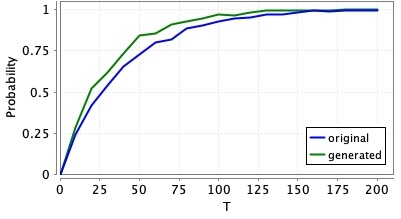
\includegraphics[scale=0.27]{example6-results.jpeg}	
	\caption{}
	\vspace{-0.25cm}
	\label{ex5-res}
	\end{wrapfigure}
The code closely resembles the one outlined in \cite{DBLP:journals/distribledger/GallettaLMV23}, with the main distinction being the greater number of lines in our generated model. 
This difference is due to the fact that certain commands could be combined, but our generation lacks the automatic capability to perform this check. While the results exhibit similarity, running simulations for the generated model takes PRISM 39.016 seconds, compared to the 22.051 seconds required for the original model.


\begin{comment}
\subsection{Problems}
\label{sec:problems}
While testing our choreographic language, we noticed that some of the case studies presented in the 
PRISM documentation \cite{PRISMdoc} cannot be modeled by using our language.
The reasons are various, in this section we try to outline the problems.

\begin{itemize}
\item \textbf{Asynchronous Leader Election}\footnote{\url{https://www.prismmodelchecker.org/casestudies/asynchronous_leader.php}}:
 processes synchronize with the same label but the conditions are different.
 We include in our language the \texttt{it-then-else} statement but we do not allow 
 the \texttt{if-then} (without the \texttt{else}). This is done because in this way, we do not 
 incur in deadlock states.
\item  \textbf{Probabilistic Broadcast Protocols}\footnote{\url{https://www.prismmodelchecker.org/casestudies/prob_broadcast.php}}:
 also in this case, the problem are the labels of the synchronizations.
 In fact, all the processes synchornize with the same label on every actions.
 This is not possible in our language, since a label is unique for every synchronization between two (or more) processes.
\item \textbf{Cyclic Server Polling System}\footnote{\url{https://www.prismmodelchecker.org/casestudies/polling.php}}:
 in this model, the processes \texttt{station$_i$} do two different things in the same state.
 More precicely, at the state 0 (\texttt{s$_i$=0}), the processes may synchornize with the process
 \texttt{server} or may change their state without any synchronization.
 In out language, this cannot be formalized since the synchronization is a branch action,
 so there should be another option with a synchronization.


\end{itemize}
\end{comment}